\documentclass[a4paper, 11pt]{article}
\usepackage{graphicx}
\usepackage{amsmath}
\usepackage[pdftex]{hyperref}
\usepackage{graphicx}
\usepackage[export]{adjustbox}
\usepackage{subcaption}
\usepackage{wrapfig}

% Lengths and indenting
\setlength{\textwidth}{16.5cm}
\setlength{\marginparwidth}{1.5cm}
\setlength{\parindent}{0cm}
\setlength{\parskip}{0.15cm}
\setlength{\textheight}{24cm}
\setlength{\oddsidemargin}{0cm}
\setlength{\evensidemargin}{\oddsidemargin}
\setlength{\topmargin}{0cm}
\setlength{\headheight}{0cm}
\setlength{\headsep}{0cm}

\renewcommand{\familydefault}{\sfdefault}

\title{Introduction to Learning and Intelligent Systems - Spring 2015}
\author{jo@student.ethz.ch\\ sakhadov@student.ethz.ch\\  stegeran@student.ethz.ch\\}
\date{\today}

\begin{document}
\maketitle
\section*{Project 1 : Regression}

The task given in the Project was to predict passenger number given time stamps and other (unknown) data features. Linear Regression (or some variant thereof) had to be used to complete the task. First, the time stamps had to be parsed to be able to use components like e.g. year, hour, and minute.

As we noticed, the most important step is feature engineering, which means transforming and combining different data features to achieve a better result. In our code, this is done in the Python Method \textit{transformFeatures}.

We noticed from the data distribution that the Y values depend greatly on the train departure hour. It should not be a big surprise as the data presented are passenger numbers.
Figure 1 shows this dependency.

\begin{figure}[h]
 
\begin{subfigure}[l]{0.5\textwidth}
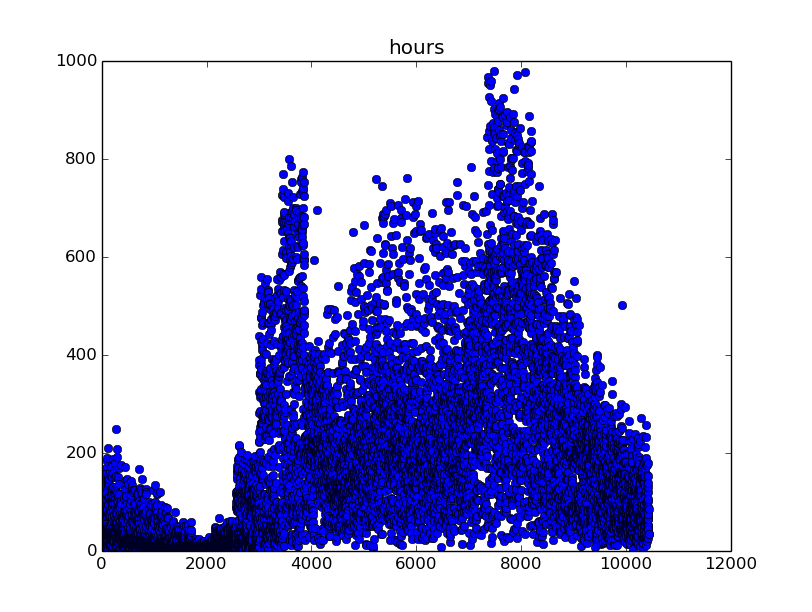
\includegraphics[width=0.9\linewidth, height=5cm]{Plots/hours} 
\caption{Given data}
\label{fig:subim1}
\end{subfigure}
\begin{subfigure}[r]{0.5\textwidth}
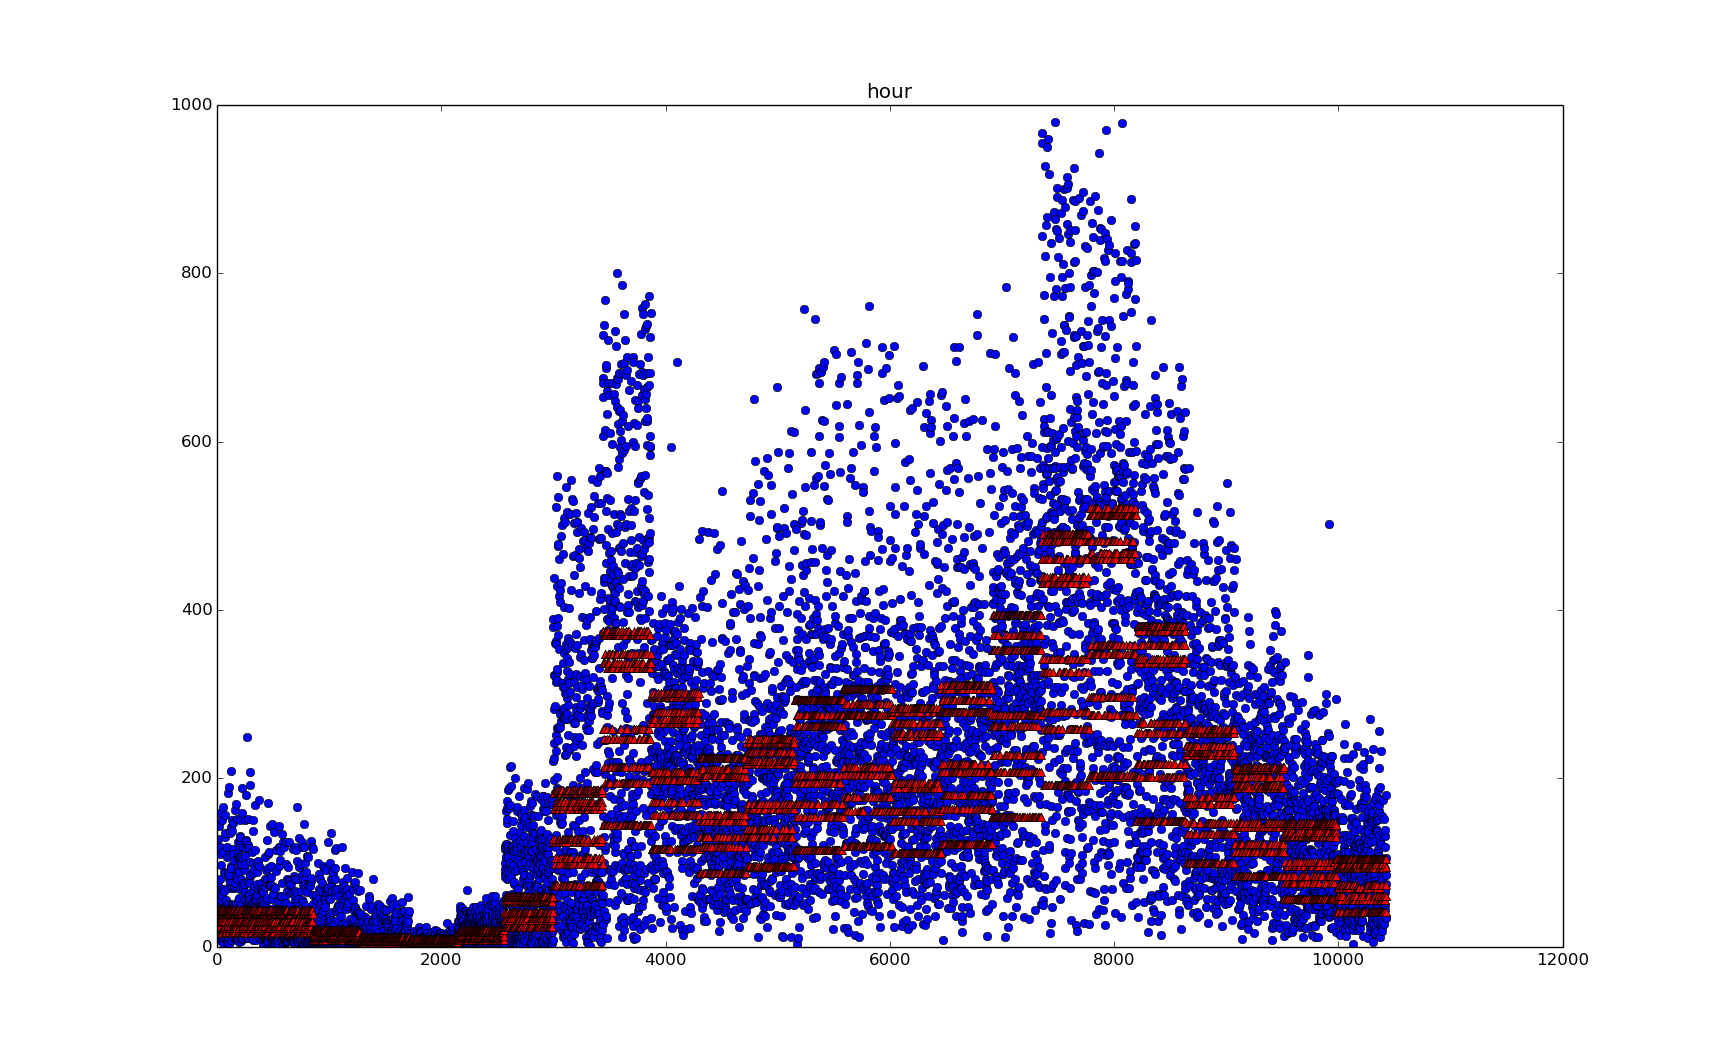
\includegraphics[width=0.9\linewidth, height=5cm]{Plots/hours_predicted}
\caption{Our resulting prediction}
\label{fig:subim2}
\end{subfigure}
 
\caption{Y values sorted by hour}
\label{fig:image2}
\end{figure}

Additionally we use other features such as month, year, day of year and the factors A-F.

 We construct our feature vectors for hour values with monomials of the degree up to 5. Using minutes did not give any gain, hours seem to be precise enough. Other features like year and month were transformed using polynomials, too.

We introduced a new True/False feature for the difference between weekends and weekdays. The working days had generally more passengers during the day than the weekends as the Figure 2 shows. We also noticed that half of the data was on the weekends. We tried to use this knowledge and weight the data points on the working days higher. However this approach did not produce much better results. 
 
Another important point to make is that the data is roughly exponentially distributed. This can be seen on Figure 2a. For the fitting we therefore took the logarithm of the values. This allowed for better linear regression and considerable predication accuracy gain. The predicted values had then to be transformed back using the exponential function in order to get the actual approximation. This step also takes care of the problem of negative values occurring in the prediction.

Combing features together we achieved further improvement. To capture the correlation between hours and other factors we produced several feature vectors consisting of the products of hour vector and other features. These vectors were also expanded to monomials of the degree up to 5. 

The last step was to normalize the feature vectors. This was done per feature vector by subtracting the mean and dividing by the standard deviation.

we tried out several variants of linear regressions employing different penalty functions, like Ridge and Lasso regression in order to amend our results. We now use Ridge regression with an alpha penalty parameter value of 1.


\begin{figure}[h]
 
\begin{subfigure}[l]{0.5\textwidth}
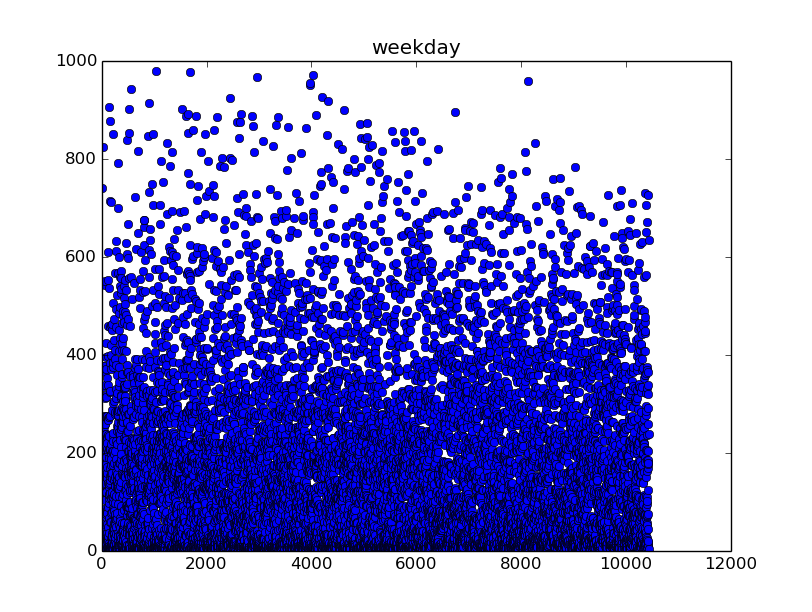
\includegraphics[width=0.9\linewidth, height=5cm]{Plots/weekdays} 
\caption{sorted by weekdays}
\label{fig:subim3}
\end{subfigure}
\begin{subfigure}[r]{0.5\textwidth}
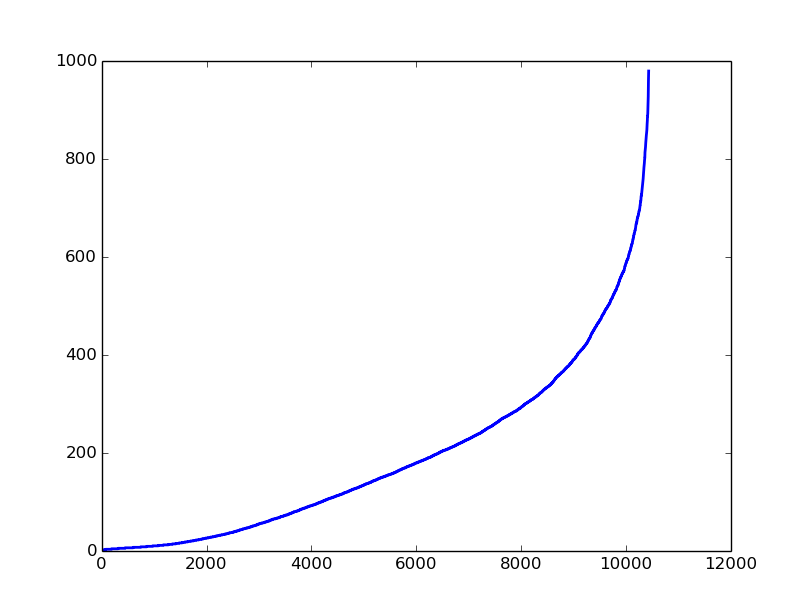
\includegraphics[width=0.9\linewidth, height=5cm]{Plots/data_sorted}
\caption{sorted by value}
\label{fig:subim4}

\end{subfigure}
\caption{Y values}
\end{figure}


\end{document}
